% ============================================================================
%  FurlPay — System Architecture (research-paper style, self-contained)
%  Compile:  pdflatex furlpay-architecture.tex   (run twice for references)
%  Requires: TikZ (ships with TeX Live / MiKTeX). No external images needed.
% ============================================================================
\documentclass[10pt,twocolumn]{article}

\usepackage[margin=0.75in]{geometry}
\usepackage{times}
\usepackage{amsmath,amssymb}
\usepackage{xcolor}
\usepackage{tikz}
\usepackage{booktabs}
\usepackage{enumitem}
\usepackage{hyperref}
\usepackage{microtype}
\usetikzlibrary{positioning,arrows.meta,shapes.geometric,calc,backgrounds,fit,shadows,shapes.multipart}

% ---- Brand palette ----------------------------------------------------------
\definecolor{neon}{HTML}{00E599}
\definecolor{neondeep}{HTML}{00A870}
\definecolor{ink}{HTML}{0B0D12}
\definecolor{slate}{HTML}{2A2F3A}
\definecolor{sky}{HTML}{0EA5E9}
\definecolor{violet}{HTML}{7C3AED}
\definecolor{amber}{HTML}{D97706}
\definecolor{rose}{HTML}{E11D48}
\definecolor{emerald}{HTML}{059669}
\definecolor{indigo}{HTML}{4F46E5}
% light fills
\definecolor{fneon}{HTML}{E5FBF3}
\definecolor{fsky}{HTML}{E0F2FE}
\definecolor{fviolet}{HTML}{EDE9FE}
\definecolor{famber}{HTML}{FEF3C7}
\definecolor{frose}{HTML}{FFE4E6}
\definecolor{femerald}{HTML}{D1FAE5}
\definecolor{findigo}{HTML}{E0E7FF}
\definecolor{fslate}{HTML}{EEF1F5}

\hypersetup{colorlinks=true, linkcolor=neondeep, urlcolor=neondeep, citecolor=neondeep}

% ---- Reusable TikZ styles ---------------------------------------------------
\tikzset{
  layer/.style   ={rounded corners=4pt, draw=#1, fill=#1!8, line width=0.9pt},
  comp/.style    ={rounded corners=3pt, draw=#1, fill=#1!12, line width=0.7pt,
                   font=\scriptsize\sffamily, align=center, minimum height=6mm, inner sep=3pt, drop shadow={opacity=0.15,shadow xshift=1pt,shadow yshift=-1pt}},
  chip/.style    ={rounded corners=6pt, draw=#1, fill=white, line width=1pt,
                   font=\scriptsize\sffamily\bfseries, text=#1, align=center, minimum height=8mm, inner sep=4pt},
  chain/.style   ={cylinder, shape border rotate=90, aspect=0.28, draw=#1, fill=#1!12,
                   font=\scriptsize\sffamily\bfseries, text=#1, align=center, minimum width=14mm, minimum height=9mm, inner sep=2pt},
  store/.style   ={cylinder, shape border rotate=90, aspect=0.22, draw=slate, fill=fslate,
                   font=\scriptsize\sffamily, align=center, minimum width=16mm, minimum height=8mm},
  actor/.style   ={rounded corners=10pt, draw=ink, fill=ink!85, text=white,
                   font=\scriptsize\sffamily\bfseries, align=center, minimum height=8mm, inner sep=4pt},
  flowarr/.style ={-{Stealth[length=2.4mm]}, line width=0.9pt},
  dashedarr/.style={-{Stealth[length=2.4mm]}, line width=0.8pt, dashed},
  steplbl/.style ={circle, draw=neondeep, fill=neon, text=ink, font=\tiny\bfseries, inner sep=1pt, minimum size=3.6mm},
}

% ============================================================================
\title{\vspace{-1.2em}\textbf{FurlPay: An On-Chain Financial Operating System\\for the Agentic Internet}\\[0.3em]
\large A System Architecture and Reference Design}
\author{FurlPay Architecture Team \\ \small FurlPay \;\textbullet\; \texttt{hello@furlpay.com} \;\textbullet\; \url{https://furlpay.com}}
\date{\small July 2026}

\begin{document}
\twocolumn[
\begin{@twocolumnfalse}
\maketitle
\begin{abstract}
\noindent
FurlPay is an open-source financial operating system that unifies stablecoin
payments, global banking, virtual-card issuing, and fractional investing behind a
single API, and extends that surface to autonomous software agents through the
\emph{x402} pay-per-call protocol. This paper documents the system's reference
architecture: a five-layer stack spanning multi-language client SDKs, a
Next.js edge/serverless API tier of thirty-nine service groups, an on-chain
settlement layer of four core smart contracts and a modular compliance suite
deployed against USDC across six blockchains, and a first-class agentic layer
exposing the platform to Model Context Protocol clients and seven agent
frameworks. We describe the payment rails (EIP-712 authorized transfers and
EIP-3009 gasless \texttt{transferWithAuthorization}), the x402 facilitator and its
hardening layer (\texttt{x402-guard}), a double-entry ledger, and the
compliance/security controls (KYC/AML, FATF Travel Rule, MPC signing). We
illustrate the design with an end-to-end agentic travel-booking flow whose every
step settles and proves on-chain.
\vspace{0.6em}
\end{abstract}
\end{@twocolumnfalse}
]

% ============================================================================
\section{Introduction}
The migration of commerce toward autonomous agents creates a settlement problem:
agents transact continuously, in small amounts, across services that neither share
accounts nor tolerate the latency of card rails. FurlPay addresses this by treating
\emph{stablecoins as the settlement primitive} and \emph{HTTP~402 as the payment
handshake}. Humans use the same platform for payments, banking, cards, and
investing; agents use it to pay per API call within enforced budgets. The entire
public surface is MIT-licensed; custody engines, fraud models, and HSM signing
policies remain in a private core.

This document is a reference architecture. Section~\ref{sec:overview} presents the
layered system; Sections~\ref{sec:sdk}--\ref{sec:api} cover the client and service
tiers; Section~\ref{sec:chain} details the on-chain rails and contracts;
Section~\ref{sec:x402} specifies the x402 agentic protocol; Section~\ref{sec:agents}
covers AI-agent integration; Section~\ref{sec:controls} covers the ledger,
compliance, and security controls; and Section~\ref{sec:flow} walks a complete
agentic booking end-to-end.

\section{Design Goals}
\begin{description}[leftmargin=1.1em,style=nextline,itemsep=1pt]
  \item[G1 One surface, many clients.] Identical client semantics and webhook
        signatures across Node, Python, Go, and Rust.
  \item[G2 Agent-native settlement.] Pay-per-call over x402 with per-agent spend
        budgets and Know-Your-Agent (KYA) trust signals.
  \item[G3 Verifiable money.] Every booking and payout produces an on-chain
        receipt; the ledger is double-entry and reversible.
  \item[G4 Compliance by construction.] KYC/AML, jurisdiction geofencing, and the
        FATF Travel Rule enforced at the policy layer and, optionally, on-chain.
  \item[G5 Zero-credential trials.] Every SDK and tool runs in a deterministic
        demo mode so integrations can be observed end-to-end without an account.
\end{description}

% ============================================================================
\section{System Overview}\label{sec:overview}
FurlPay is organized as five cooperating layers (Figure~\ref{fig:stack}): the
\textbf{client \& agent} layer, the \textbf{SDK} layer, the \textbf{API \&
middleware} layer, the \textbf{service} layer, and the \textbf{settlement \& data}
layer. Requests enter through language SDKs or the MCP server, cross an
authentication/compliance middleware, fan out to domain services, and settle on
one of six chains while being journaled into a double-entry ledger.

\begin{figure*}[t]
\centering
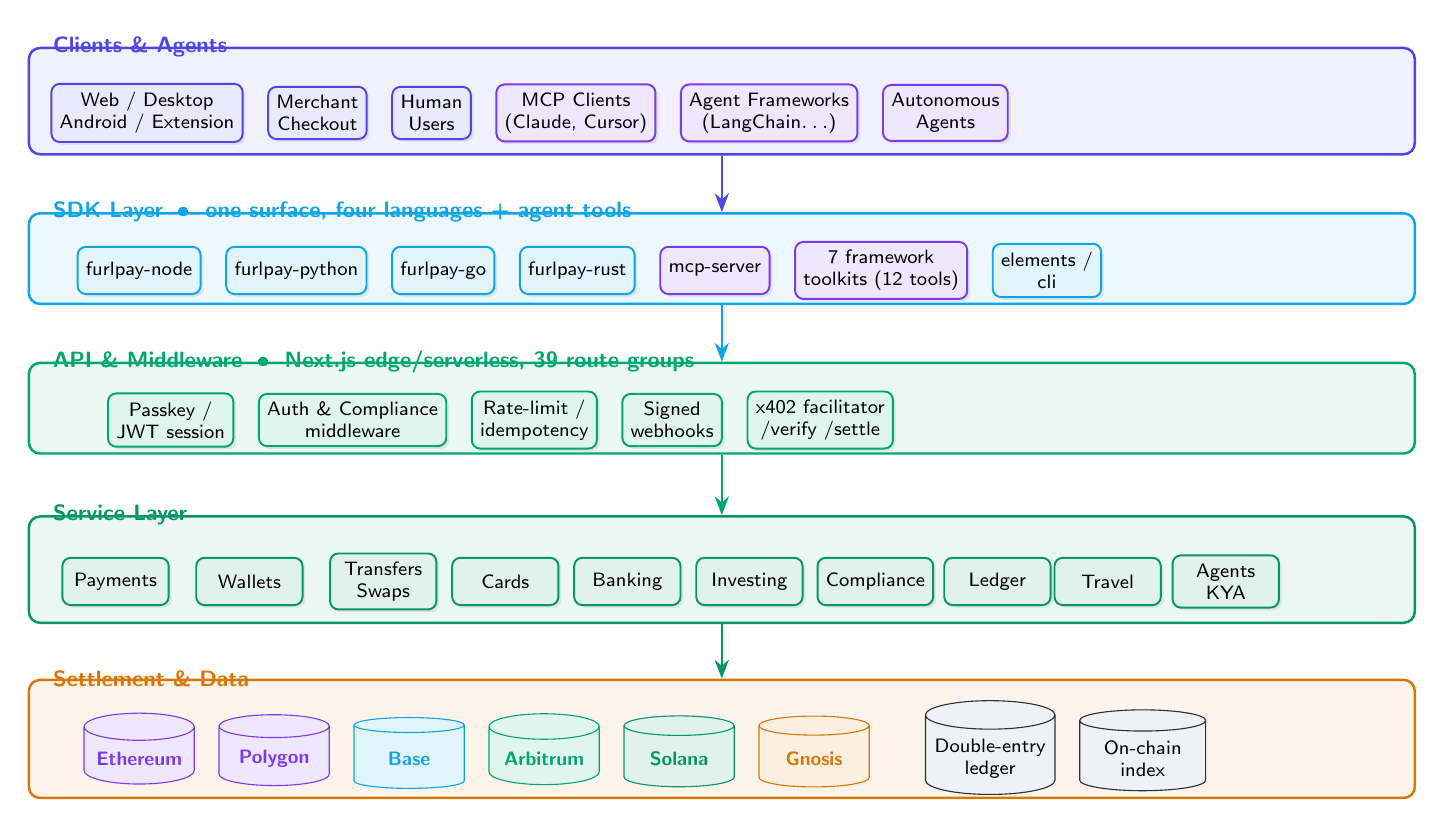
\begin{tikzpicture}[node distance=3mm]
% ---- Layer 1: clients & agents
\node[layer=indigo, minimum width=17.6cm, minimum height=1.35cm] (L1) at (0,0) {};
\node[anchor=west, font=\footnotesize\sffamily\bfseries, text=indigo] at ([xshift=2mm]L1.north west) {Clients \& Agents};
\node[comp=indigo] (webapp)  at (-7.3,-0.15) {Web / Desktop\\Android / Extension};
\node[comp=indigo, right=of webapp] (merch) {Merchant\\Checkout};
\node[comp=indigo, right=of merch] (human) {Human\\Users};
\node[comp=violet, right=of human] (mcpc)  {MCP Clients\\(Claude, Cursor)};
\node[comp=violet, right=of mcpc] (frame)  {Agent Frameworks\\(LangChain$\ldots$)};
\node[comp=violet, right=of frame] (agent) {Autonomous\\Agents};

% ---- Layer 2: SDKs
\node[layer=sky, minimum width=17.6cm, minimum height=1.15cm] (L2) at (0,-2.0) {};
\node[anchor=west, font=\footnotesize\sffamily\bfseries, text=sky] at ([xshift=2mm]L2.north west) {SDK Layer \;\textbullet\; one surface, four languages + agent tools};
\node[comp=sky] (sn) at (-7.4,-2.15) {furlpay-node};
\node[comp=sky, right=of sn] (sp) {furlpay-python};
\node[comp=sky, right=of sp] (sg) {furlpay-go};
\node[comp=sky, right=of sg] (sr) {furlpay-rust};
\node[comp=violet, right=of sr] (mcps) {mcp-server};
\node[comp=violet, right=of mcps] (tools) {7 framework\\toolkits (12 tools)};
\node[comp=sky, right=of tools] (elem) {elements /\\cli};

% ---- Layer 3: API & middleware
\node[layer=neondeep, minimum width=17.6cm, minimum height=1.15cm] (L3) at (0,-3.9) {};
\node[anchor=west, font=\footnotesize\sffamily\bfseries, text=neondeep] at ([xshift=2mm]L3.north west) {API \& Middleware \;\textbullet\; Next.js edge/serverless, 39 route groups};
\node[comp=neondeep] (auth) at (-7.0,-4.05) {Passkey /\\JWT session};
\node[comp=neondeep, right=of auth] (mw) {Auth \& Compliance\\middleware};
\node[comp=neondeep, right=of mw] (rl) {Rate-limit /\\idempotency};
\node[comp=neondeep, right=of rl] (wh) {Signed\\webhooks};
\node[comp=neondeep, right=of wh] (x4) {x402 facilitator\\/verify /settle};

% ---- Layer 4: services
\node[layer=emerald, minimum width=17.6cm, minimum height=1.35cm] (L4) at (0,-5.95) {};
\node[anchor=west, font=\footnotesize\sffamily\bfseries, text=emerald] at ([xshift=2mm]L4.north west) {Service Layer};
\foreach \name/\x in {Payments/-7.7, Wallets/-6.0, {Transfers\\Swaps}/-4.3, Cards/-2.75, Banking/-1.2, Investing/0.35, Compliance/1.95, Ledger/3.5, Travel/4.9, {Agents\\KYA}/6.4} {
  \node[comp=emerald, minimum width=1.35cm] at (\x,-6.1) {\name};
}

% ---- Layer 5: settlement & data
\node[layer=amber, minimum width=17.6cm, minimum height=1.5cm] (L5) at (0,-8.1) {};
\node[anchor=west, font=\footnotesize\sffamily\bfseries, text=amber] at ([xshift=2mm]L5.north west) {Settlement \& Data};
\node[chain=violet] (c1) at (-7.4,-8.35) {Ethereum};
\node[chain=violet, right=3mm of c1] (c2) {Polygon};
\node[chain=sky, right=3mm of c2] (c3) {Base};
\node[chain=neondeep, right=3mm of c3] (c4) {Arbitrum};
\node[chain=emerald, right=3mm of c4] (c5) {Solana};
\node[chain=amber, right=3mm of c5] (c6) {Gnosis};
\node[store, right=7mm of c6] (led) {Double-entry\\ledger};
\node[store, right=3mm of led] (idx) {On-chain\\index};

% ---- vertical connective arrows
\draw[flowarr, indigo]   (L1) -- (L2);
\draw[flowarr, sky]      (L2) -- (L3);
\draw[flowarr, neondeep] (L3) -- (L4);
\draw[flowarr, emerald]  (L4) -- (L5);
\end{tikzpicture}
\caption{The five-layer FurlPay architecture. Requests descend from clients and
agents through language SDKs and the MCP server, cross an authentication and
compliance middleware, fan out across domain services, and settle in USDC on one
of six chains while being journaled into a double-entry ledger and on-chain index.}
\label{fig:stack}
\end{figure*}

% ============================================================================
\section{Client \& SDK Layer}\label{sec:sdk}
FurlPay ships four server-side SDKs---\texttt{furlpay-node},
\texttt{furlpay-python}, \texttt{furlpay-go}, \texttt{furlpay-rust}---that expose
an identical resource surface (\texttt{wallets}, \texttt{payments},
\texttt{transfers}, \texttt{cards}, \texttt{banking}, \texttt{investing},
\texttt{swaps}, \texttt{x402}, \texttt{webhooks}) and a shared HMAC-SHA256 webhook
signature scheme (\texttt{t=$\langle$unix$\rangle$,v1=$\langle$hex$\rangle$} with a
five-minute replay window). Client-facing surfaces include \texttt{elements}
(embeddable React checkout/card widgets), the \texttt{cli}
(\emph{stripe-cli for stablecoins}: webhook forwarding and test events), and a
Chrome MV3 \texttt{extension}.

For agents, the same twelve-tool surface (pay, invest, transfer, swap, and
autonomous x402 payment within a budget) is re-exported to seven frameworks:
LangChain, LlamaIndex, CrewAI, the OpenAI Agents SDK, Pydantic AI, the Vercel AI
SDK, and Mastra. Each toolkit is a thin adapter over a shared REST client with a
demo-mode fallback (G5).

\section{API \& Middleware Layer}\label{sec:api}
The API is a Next.js application of thirty-nine route groups. A single edge
middleware verifies the passkey-minted session JWT, classifies each path as public
or protected, and applies the compliance gate before any handler runs; agent and
webhook routes authenticate by signature rather than session (RFC~9421 for agents,
Ed25519 for Discord, HMAC for webhooks). Representative groups include
\texttt{payments}, \texttt{wallets}, \texttt{cards}, \texttt{banking},
\texttt{investing}, \texttt{swaps}, \texttt{offramp}, \texttt{escrow},
\texttt{compliance}, \texttt{ledger}, \texttt{chain}, and \texttt{x402}.

% ============================================================================
\section{On-Chain Rails}\label{sec:chain}
FurlPay treats \textbf{USDC as the unit of settlement} and supports the stablecoin
set \{USDC, USDT, EURC, PYUSD, DAI\} across six chains
(Table-free; see Figure~\ref{fig:rails}). The canonical smart contracts are
deployed on \textbf{Arbitrum One}; Base and Solana serve x402 settlement.

\begin{figure}[t]
\centering
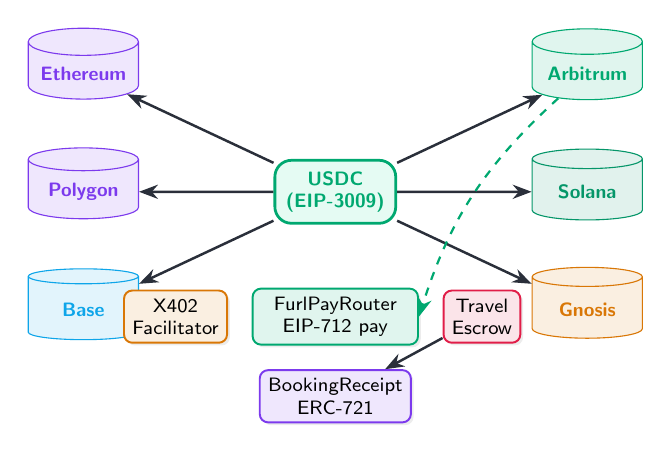
\begin{tikzpicture}[node distance=3mm]
% USDC hub
\node[chip=neondeep, fill=fneon] (usdc) at (0,0) {USDC\\(EIP-3009)};
% chains ring
\node[chain=violet]  (e) at (-3.2,1.5) {Ethereum};
\node[chain=violet]  (p) at (-3.2,0.0) {Polygon};
\node[chain=sky]     (b) at (-3.2,-1.5) {Base};
\node[chain=neondeep](a) at (3.2,1.5)  {Arbitrum};
\node[chain=emerald] (s) at (3.2,0.0)  {Solana};
\node[chain=amber]   (g) at (3.2,-1.5) {Gnosis};
\foreach \n in {e,p,b,a,s,g} { \draw[flowarr, slate] (usdc) -- (\n); }
% contracts cluster on Arbitrum
\node[comp=neondeep, below=8mm of usdc, minimum width=2.1cm] (router) {FurlPayRouter\\EIP-712 pay};
\node[comp=amber, left=3mm of router] (fac) {X402\\Facilitator};
\node[comp=rose, right=3mm of router] (esc) {Travel\\Escrow};
\node[comp=violet, below=3mm of router] (nft) {BookingReceipt\\ERC-721};
\draw[dashedarr, neondeep] (a) to[bend right=15] (router.east);
\draw[flowarr, slate] (esc) -- (nft);
\end{tikzpicture}
\caption{On-chain rails. USDC (Circle's EIP-3009 token) is the settlement
primitive across six chains; the canonical FurlPay contracts---payment router,
x402 facilitator, travel escrow, and the ERC-721 booking receipt---are deployed on
Arbitrum One.}
\label{fig:rails}
\end{figure}

\subsection{Core contracts}
\begin{description}[leftmargin=1em,style=nextline,itemsep=2pt]
  \item[\texttt{FurlPayRouter}] The USDC payment rail. A payer signs an EIP-712
        \texttt{Payment} authorization off-chain (via
        \texttt{POST\ /api/payments/create}); a relayer submits it. The payer is
        debited \texttt{amount}, the
        recipient receives \texttt{amount}$-$\texttt{fee}, and the 0.5\% fee accrues
        to the treasury. Each authorization carries a single-use nonce and a
        \texttt{deadline}; \texttt{Pausable} and \texttt{ReentrancyGuard} apply.
  \item[\texttt{X402Facilitator}] A non-custodial forwarder over USDC's EIP-3009
        \texttt{transferWithAuthorization}. It never holds funds or keys---it
        verifies the token-domain signature, forwards the gasless transfer, and
        indexes the settlement for discovery.
  \item[\texttt{FurlPayEscrow}] Travel-booking escrow. The traveler funds a booking
        in USDC; funds release to the provider on a check-in oracle confirmation,
        refund to the traveler before the cancellation deadline, or release after a
        grace period so providers are never held hostage.
  \item[\texttt{BookingReceipt}] An ERC-721 proof-of-purchase minted by the escrow
        when a booking is funded; \texttt{tokenId} equals the booking id, so a
        receipt is verifiable directly from the booking reference.
\end{description}

A modular \textbf{compliance suite} (\texttt{PolicyManager},
\texttt{AttestationRegistry}, \texttt{SanctionsRegistry}/\texttt{SanctionsCheck},
\texttt{SourceOfFundsCheck}, \texttt{ComplianceEscrow},
\texttt{X402PolicyWrapper}) allows policy checks---sanctions, source-of-funds,
attestations---to gate settlement on-chain when a jurisdiction requires it.

% ============================================================================
\section{The x402 Agentic Payment Protocol}\label{sec:x402}
x402 turns HTTP~402 into a payment handshake: an unpaid request receives a 402 with
a machine-readable price challenge; the client settles through a facilitator and
retries with an \texttt{X-PAYMENT} header. Figure~\ref{fig:x402} shows the flow.
FurlPay operates the first \emph{Solana-native} facilitator and hardens it with
\texttt{x402-guard}, which closes five known facilitator flaw classes:
request-binding (F1), atomic nonce claim against duplicate settlement (F2),
pessimistic reserve-commit against allowance overdraft (F3), settlement-capacity
limiting against denial-of-settlement (F4), and EWMA adaptive pricing against
hidden-compute free-riding (F5).

\begin{figure}[t]
\centering
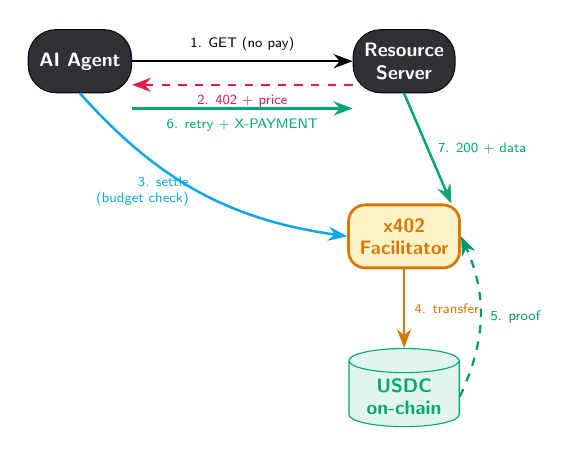
\begin{tikzpicture}[node distance=6mm and 14mm]
\node[actor] (ag) {AI Agent};
\node[actor, right=28mm of ag] (rs) {Resource\\Server};
\node[chip=amber, fill=famber, below=14mm of rs] (fa) {x402\\Facilitator};
\node[chain=neondeep, below=10mm of fa] (ch) {USDC\\on-chain};

\draw[flowarr] (ag.east|-ag) -- node[above,font=\tiny\sffamily]{1. GET (no pay)} (rs.west|-ag);
\draw[dashedarr, rose] ([yshift=-3mm]rs.west) -- node[below,font=\tiny\sffamily]{2. 402 + price} ([yshift=-3mm]ag.east);
\draw[flowarr, sky] (ag.south) to[bend right=20] node[left,font=\tiny\sffamily,align=right]{3. settle\\(budget check)} (fa.west);
\draw[flowarr, amber] (fa) -- node[right,font=\tiny\sffamily]{4. transfer} (ch);
\draw[dashedarr, emerald] (ch.east) to[bend right=25] node[right,font=\tiny\sffamily]{5. proof} (fa.east);
\draw[flowarr, neondeep] ([yshift=-6mm]ag.east) -- node[below,font=\tiny\sffamily,align=center]{6. retry + X-PAYMENT} ([yshift=-6mm]rs.west);
\draw[flowarr, neondeep] (rs.south) -- node[right,font=\tiny\sffamily]{7. 200 + data} ([xshift=6mm]rs.south|-fa.north);
\end{tikzpicture}
\caption{The x402 pay-per-call handshake. An unpaid request (1) is answered with a
402 price challenge (2); the agent settles through the facilitator within its spend
budget (3--5) and retries with an \texttt{X-PAYMENT} header (6), receiving the
gated resource (7). \texttt{x402-guard} enforces atomicity and capacity at steps
3--5.}
\label{fig:x402}
\end{figure}

% ============================================================================
\section{AI-Agent Integration}\label{sec:agents}
FurlPay exposes two agent entry points (Figure~\ref{fig:agents}): a Model Context
Protocol server (\texttt{@furlpay/mcp-server}, plus a dedicated
\texttt{travel-mcp}) that any MCP client can discover, and framework toolkits that
bind the twelve-tool surface into each framework's native tool abstraction. An
\texttt{agent-trust} layer provides Ed25519 agent identity and Know-Your-Agent
signals, and every agent operates under a server-enforced spend budget.

\begin{figure}[t]
\centering
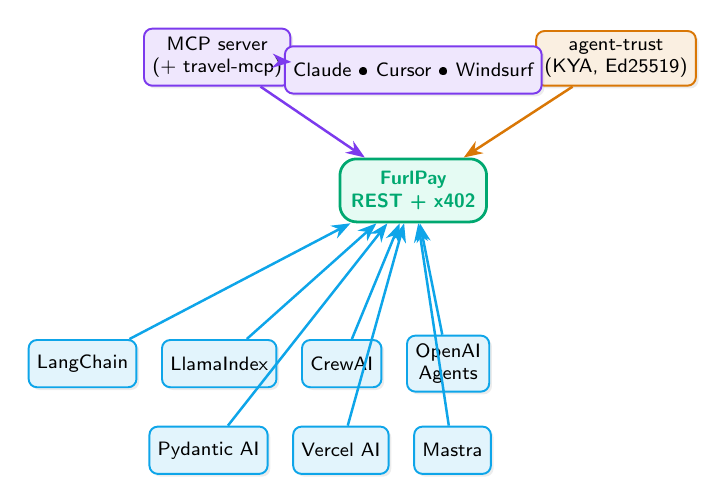
\begin{tikzpicture}[node distance=3mm]
\node[chip=neondeep, fill=fneon] (core) at (0,0) {FurlPay\\REST + x402};
\node[comp=violet, above left=9mm and 6mm of core] (mcp) {MCP server\\(+ travel-mcp)};
\node[comp=amber, above right=9mm and 6mm of core] (trust) {agent-trust\\(KYA, Ed25519)};
% framework fan
\node[comp=sky] (f1) at (-4.2,-2.2) {LangChain};
\node[comp=sky, right=of f1] (f2) {LlamaIndex};
\node[comp=sky, right=of f2] (f3) {CrewAI};
\node[comp=sky, right=of f3] (f4) {OpenAI\\Agents};
\node[comp=sky] (f5) at (-2.6,-3.3) {Pydantic AI};
\node[comp=sky, right=of f5] (f6) {Vercel AI};
\node[comp=sky, right=of f6] (f7) {Mastra};
\foreach \f in {f1,f2,f3,f4,f5,f6,f7} { \draw[flowarr, sky] (\f) -- (core); }
\draw[flowarr, violet] (mcp) -- (core);
\draw[flowarr, amber] (trust) -- (core);
\node[comp=violet, above=8mm of core] (clients) {Claude \textbullet\ Cursor \textbullet\ Windsurf};
\draw[flowarr, violet] (clients) -- (mcp);
\end{tikzpicture}
\caption{Agent integration. The twelve-tool surface reaches agents through an MCP
server (for Claude/Cursor/Windsurf) and seven framework toolkits, gated by an
\texttt{agent-trust} Know-Your-Agent layer and per-agent spend budgets.}
\label{fig:agents}
\end{figure}

% ============================================================================
\section{Ledger, Compliance \& Security}\label{sec:controls}
\textbf{Ledger.} \texttt{@furlpay/ledger} implements an immutable double-entry
journal: every movement posts balanced debits and credits, balances are derived,
and corrections are reversals rather than mutations---so the trial balance always
proves the books balance, and on-chain settlement is mirrored one-to-one into the
journal.

\textbf{Compliance.} \texttt{@furlpay/compliance} centralizes KYC/AML, the
MiCA/GENIUS and FCA geofence rules, a jurisdiction/tier engine, and FATF Travel
Rule messaging; the on-chain compliance suite optionally enforces the same policies
at settlement.

\textbf{Security.} \texttt{@furlpay/security} provides 2-of-2 MPC signing, RFC~6238
TOTP, step-up MFA, and device/behavioral signals; \texttt{account-kit} deploys
Safe/ERC-4337 smart accounts with a paymaster and time-locked escrow. Public
packages are the audited surface; custody, fraud models, and HSM policies stay
private.

% ============================================================================
\section{End-to-End Flow: Agentic Travel Booking}\label{sec:flow}
Figure~\ref{fig:flow} traces a complete booking. An agent discovers inventory via
the travel MCP, the escrow is funded in USDC, an ERC-721 receipt is minted, the
check-in oracle releases funds to the provider, and the ledger and on-chain index
record every step---yielding a fully auditable trail from intent to settlement.

\begin{figure*}[t]
\centering
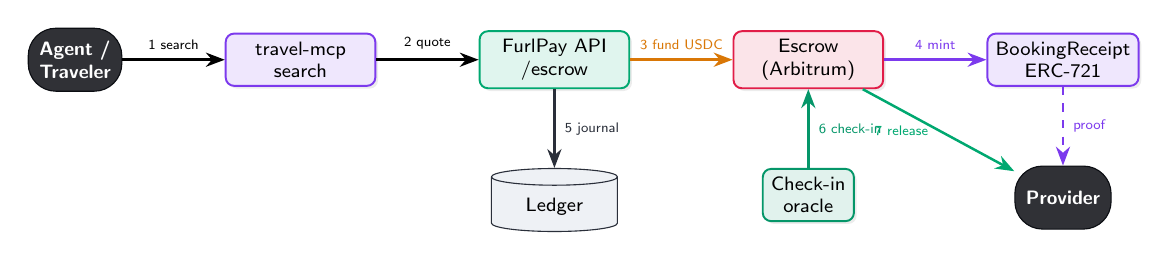
\begin{tikzpicture}[node distance=7mm and 13mm]
\node[actor] (ag) {Agent /\\Traveler};
\node[comp=violet, right=of ag, minimum width=1.9cm] (mcp) {travel-mcp\\search};
\node[comp=neondeep, right=of mcp, minimum width=1.9cm] (api) {FurlPay API\\/escrow};
\node[comp=rose, right=of api, minimum width=1.9cm] (esc) {Escrow\\(Arbitrum)};
\node[comp=violet, right=of esc, minimum width=1.9cm] (nft) {BookingReceipt\\ERC-721};
\node[store, below=10mm of api] (led) {Ledger};
\node[comp=emerald, below=10mm of esc] (oracle) {Check-in\\oracle};
\node[actor, below=10mm of nft] (prov) {Provider};

\draw[flowarr] (ag) -- node[above,font=\tiny\sffamily]{1 search} (mcp);
\draw[flowarr] (mcp) -- node[above,font=\tiny\sffamily]{2 quote} (api);
\draw[flowarr, amber] (api) -- node[above,font=\tiny\sffamily]{3 fund USDC} (esc);
\draw[flowarr, violet] (esc) -- node[above,font=\tiny\sffamily]{4 mint} (nft);
\draw[flowarr, slate] (api) -- node[right,font=\tiny\sffamily]{5 journal} (led);
\draw[flowarr, emerald] (oracle) -- node[right,font=\tiny\sffamily]{6 check-in} (esc);
\draw[flowarr, neondeep] (esc) -- node[left,font=\tiny\sffamily]{7 release} (prov);
\draw[dashedarr, violet] (nft) -- node[right,font=\tiny\sffamily]{proof} (prov);
\end{tikzpicture}
\caption{Agentic travel booking end-to-end. Search (1--2) and USDC escrow funding
(3) precede receipt minting (4) and ledger journaling (5); the check-in oracle (6)
releases escrow to the provider (7). Every step is provable from the on-chain
booking receipt.}
\label{fig:flow}
\end{figure*}

% ============================================================================
\section{Conclusion}
FurlPay demonstrates that a single open API can serve human financial primitives
and autonomous agent settlement without compromising either. By anchoring on
stablecoins, EIP-712/EIP-3009 authorized transfers, and the x402 handshake---and by
pairing them with a double-entry ledger, a modular compliance suite, and a hardened
facilitator---the platform makes agentic commerce both practical and auditable. The
public packages are MIT-licensed and run in demo mode with zero credentials,
lowering the barrier from evaluation to first payment.

% ---- References -------------------------------------------------------------
\section*{References}
\small
\begin{enumerate}[leftmargin=1.4em,itemsep=0pt]
  \item x402 Protocol Specification, Linux Foundation, 2026.
  \item EIP-3009: Transfer With Authorization (Circle USDC / FiatTokenV2).
  \item EIP-712: Typed Structured Data Hashing and Signing.
  \item ERC-4337: Account Abstraction via Entry Point Contracts.
  \item Model Context Protocol (MCP) Specification, Anthropic, 2025.
  \item FATF Recommendation 16 (the ``Travel Rule'').
  \item MiCA (EU 2023/1114) and the U.S. GENIUS Act stablecoin frameworks.
  \item \emph{x402-guard}: Facilitator-layer hardening for agentic payments (this work).
\end{enumerate}

\end{document}
